\documentclass{beamer}
% requres pygmentize to be installed on system
% also requires you to use -shell-escape flag
% when compiling document
\usepackage{minted}
% Alows me to use images in my docs
\usepackage{graphicx}
% Provides decent unicode support in case
% you don't use a unicode compatable latex
% comiler
\usepackage[utf8]{inputenc}
% these allow me to split up text into
% two collums in a nice manner
\usepackage{longtable, multicol}
% Allows better math stuff
\usepackage{amsmath}

% removes navigation button from bottom of each
% page of the presentation
\setbeamertemplate{navigation symbols}{}

% \LaTeX is a macro that prints the LaTeX symbol
\title{\LaTeX}
\subtitle{lay-teck}
\author{Some Guy}
\institute{Linux@APP}
% sets the date to whatever it is when the
% document is compiled
% you can also give it text ex. 
% 1/23/17, or  Wed. FEB 4, 2100
\date{\today}
 
\begin{document}
% Page 1 of Presentation
% is just a title page
\frame{\titlepage}
% Page 2
% explains what latex is
\begin{frame}
\frametitle{What is \LaTeX?}
LaTeX is a typesetting system, desgned to prevent the document writer from screwing everything up.
Latex is acutaly a collection of macros built ontop of TeX to make it useable for document writers, LaTeX. Instead of visually formatting your text, you enter your document text intertwined with LaTeX commands in a text file. You then run TeX to produce formatted output, such as a PDF file. Thus, in contrast to standard word processors, your document is a separate file that does not pretend to be a representation of the final typeset output, and so can be easily edited and manipulated. 

\end{frame}
% Page 3
% talks about common types of documents
% frames need to be fragile when there
% contents need to be interpreted diffrently
% like useing certain types of formating
\begin{frame}[fragile]
\frametitle{Types of documents.}
% spaces out the name of the document type
% and the description of the document type
% those two lines matched up unintentionaly
\renewcommand*{\arraystretch}{1.4}
% acutaly creates a table with two seperate colums
\begin{longtable}{l p{3 in}}
article: &     For articles in scientific journals, presentations, short reports, program documentation, invitations, ... \\
report: &      For longer reports containing several chapters, small books, thesis. \\
book: &        For real books. \\
memoir: &      It is based on the book class, but it contains lots of packages not imported by default. \\
letter: &      For writing letters. \\
beamer: &      For writing presentations (like this beamer). \\
\end{longtable}
\end{frame}

% Page 4
\begin{frame}[fragile]
\frametitle{A frame}
% \verb is used to tell LaTeX not to
% interprite text this is an inline example.
{\LaTeX} or \verb|\LaTeX|
\begin{multicols}{2}
\begin{minted}{latex}
\begin{verbatim}
\documentclass{article}
\title{A paper on how to
write papers.}
\date{2018-02-22}
\author{Andrew Pobrica}
\begin{document}
\maketitle
\pagenumbering{gobble}
\newpage
\tableofcontents
\newpage
\pagenumbering{arabic}

\section{Section}
Hello World!
\subsection{Subsection}
Stucturing a document is easy!
\subsubsection{Subsubsection}
More text.
\paragraph{Paragraph}
Some more text.
\subparagraph{Subparagraph}
    Even more text.
\section{Another section}
\end{document}
\end{verbatim}
\end{minted}
\end{multicols}
\end{frame}
% Page 5
% Python3 code
\begin{frame}[fragile]

% must install pygments for minted to work can be 2 or 3
% run latex compiler with -shell-escape as well
\begin{minted}{python3}

#Leibniz formula

pi = 0
x = 0
iterations = 10000
try:
        for x in range(iterations):
                pi = pi + 2 / ((4*x+1) * (4*x+3))
        print(pi*4)

except KeyboardInterrupt:
        print(x)
        print(pi*4)


\end{minted}

\end{frame}
%Page 6
% amsmath is used for this
\begin{frame}[fragile]
\begin{align*}
\sin A \cos B &= \frac{1}{2}\left[ \sin(A+B)+\sin(A+B) \right] \\
\sin A \sin B &= \frac{1}{2}\left[ \sin(A+B)-\cos(A+B) \right] \\
\cos A \cos B &= \frac{1}{2}\left[ \cos(A+B)+\cos(A+B) \right] \\
\end{align*}

\end{frame}
% Page 7
\begin{frame}
tlmgr update --list

tlmgr update --self

tlmgr update --all

tlmgr uninstall
\begin{figure}{Fig. 1: I got this off of reddit.}
\centering
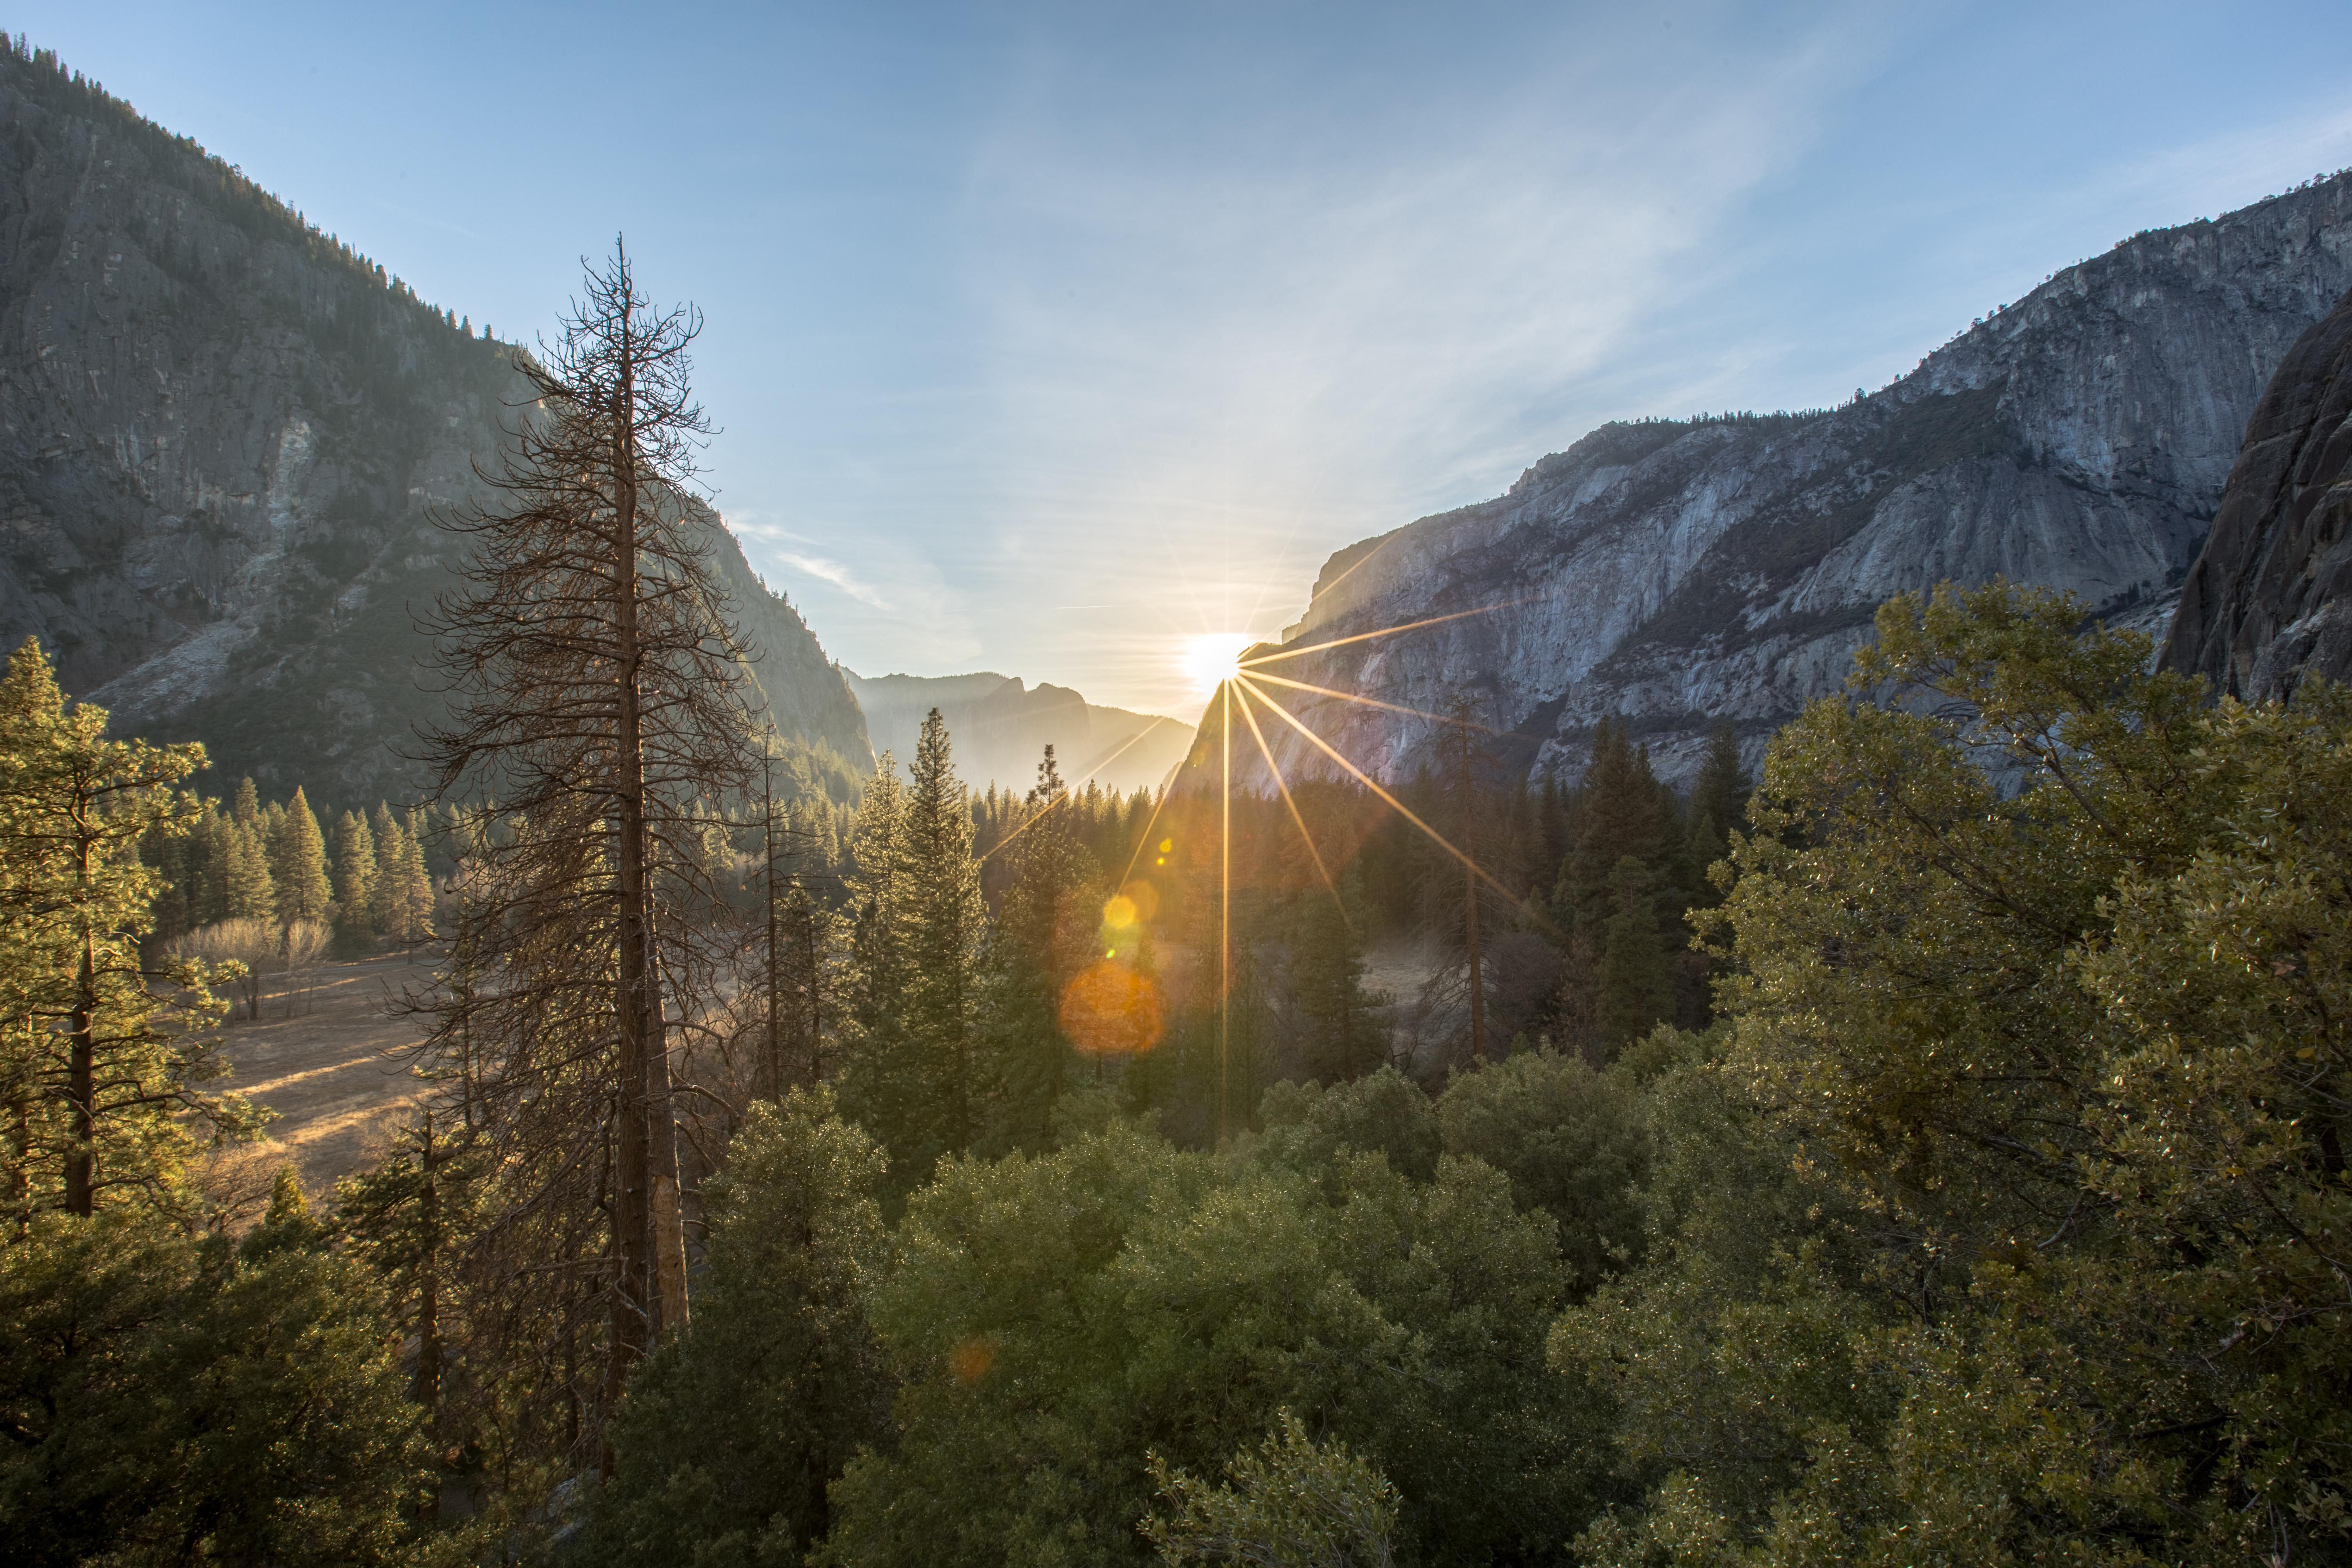
\includegraphics[height=2.5in]{picture1}
\end{figure}
\end{frame}
% Page 8
% bash stuff
\begin{frame}[fragile]
%input adds text from outside document to your latex
% document if it contains latex code it is evaluated.
\input{cowsay}
\end{frame}
%Page 9
\begin{frame}[fragile]
\begin{minted}{latex}
\LaTeX
\end{minted}
\end{frame}

\end{document}
